%!TEX root = ../paper.tex

\begin{figure*}
	\centering
	\beforeFinalVersion{Remove ticks and labels.}
	%!TEX root = ../paper.tex
%Ferdosi Sets 1
\begin{subfigure}{0.23\textwidth}
	\centering
	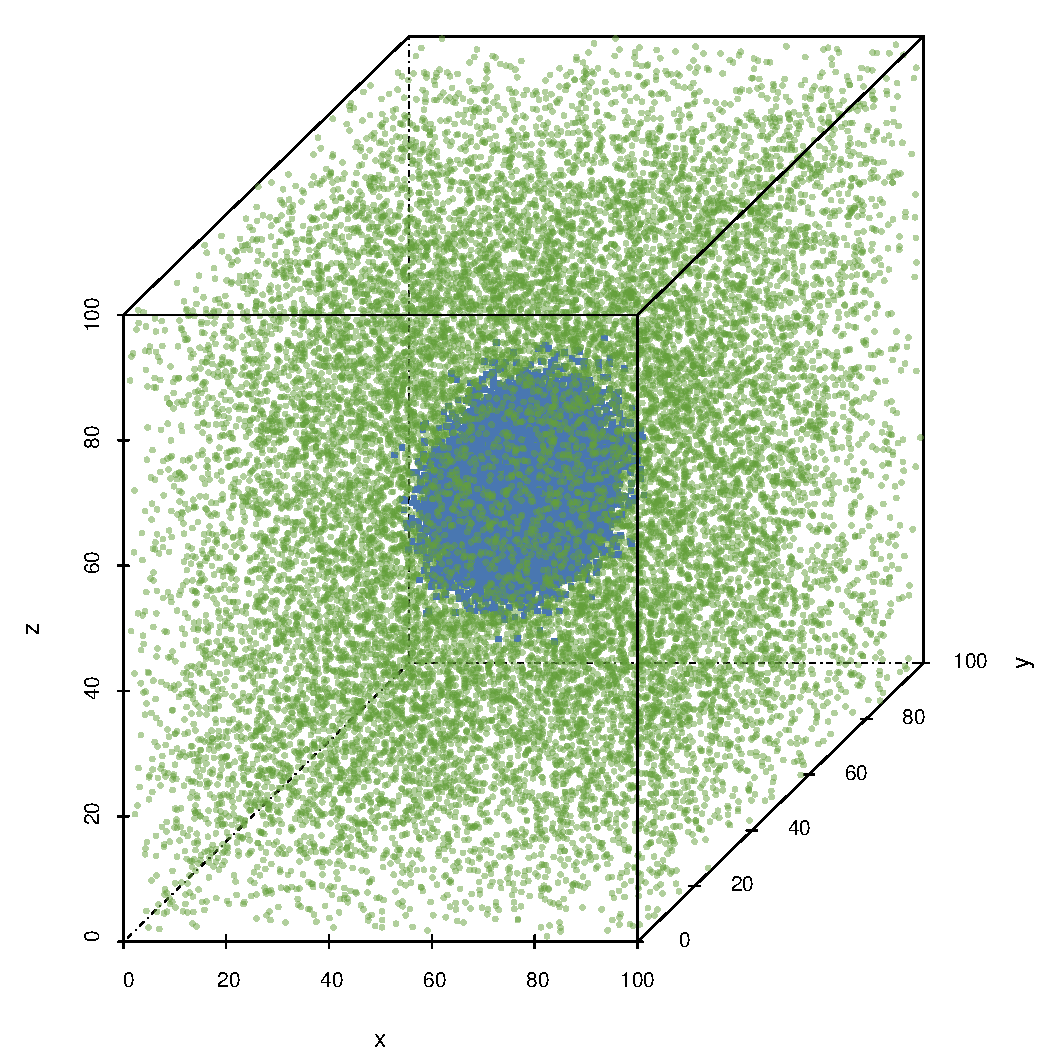
\includegraphics[width=\textwidth]{experiment/img/datasetplot_ferdosi_1_60000}
	\caption{Set \ferdosiOne}
	\label{fig:3:simulated:datasets:ferdosi1}
\end{subfigure}
% Baakman 1	
\begin{subfigure}{0.23\textwidth}
	\centering
	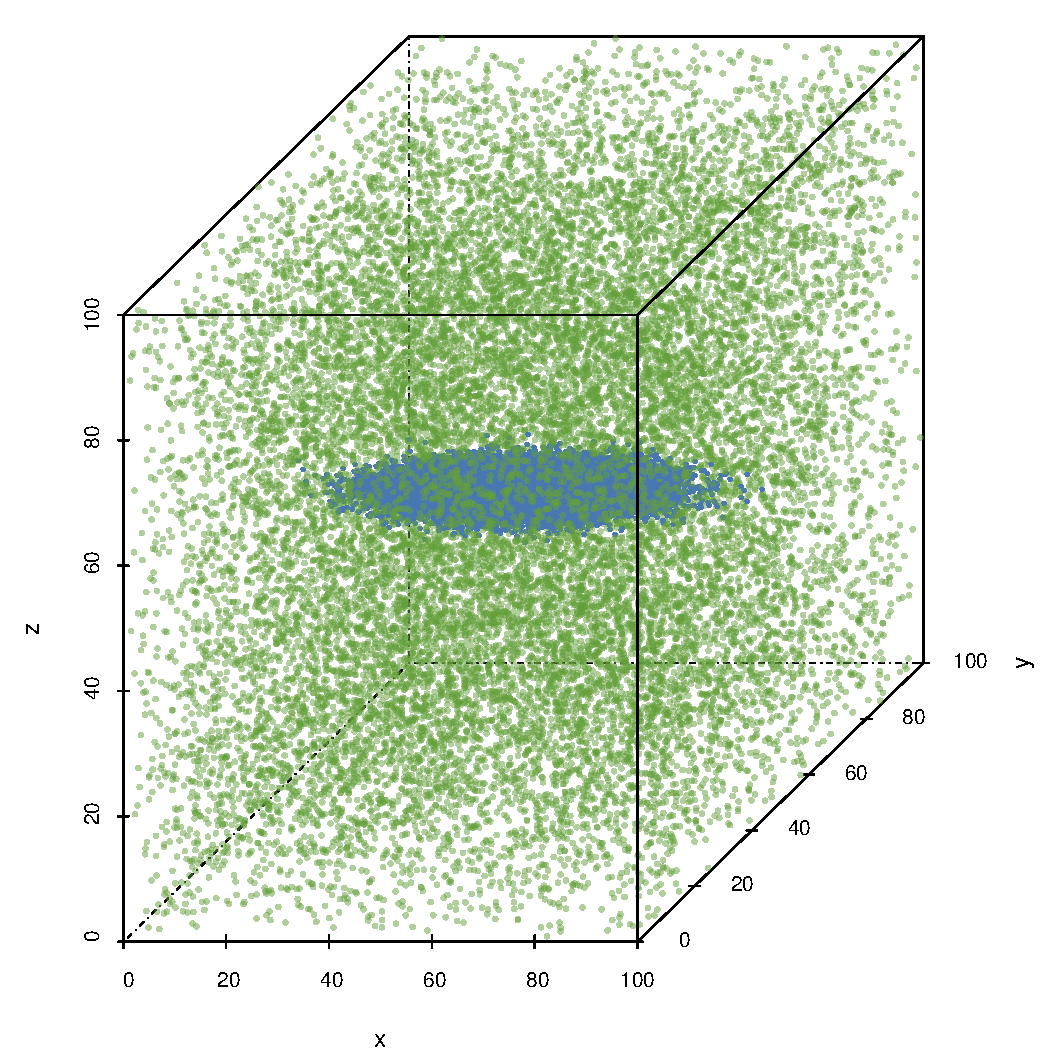
\includegraphics[width=\textwidth]{experiment/img/datasetplot_baakman_1_60000}
	\caption{Set \baakmanOne}
	\label{fig:3:simulated:datasets:baakman1}
\end{subfigure}
% Baakman 4
\begin{subfigure}{0.23\textwidth}
	\centering
	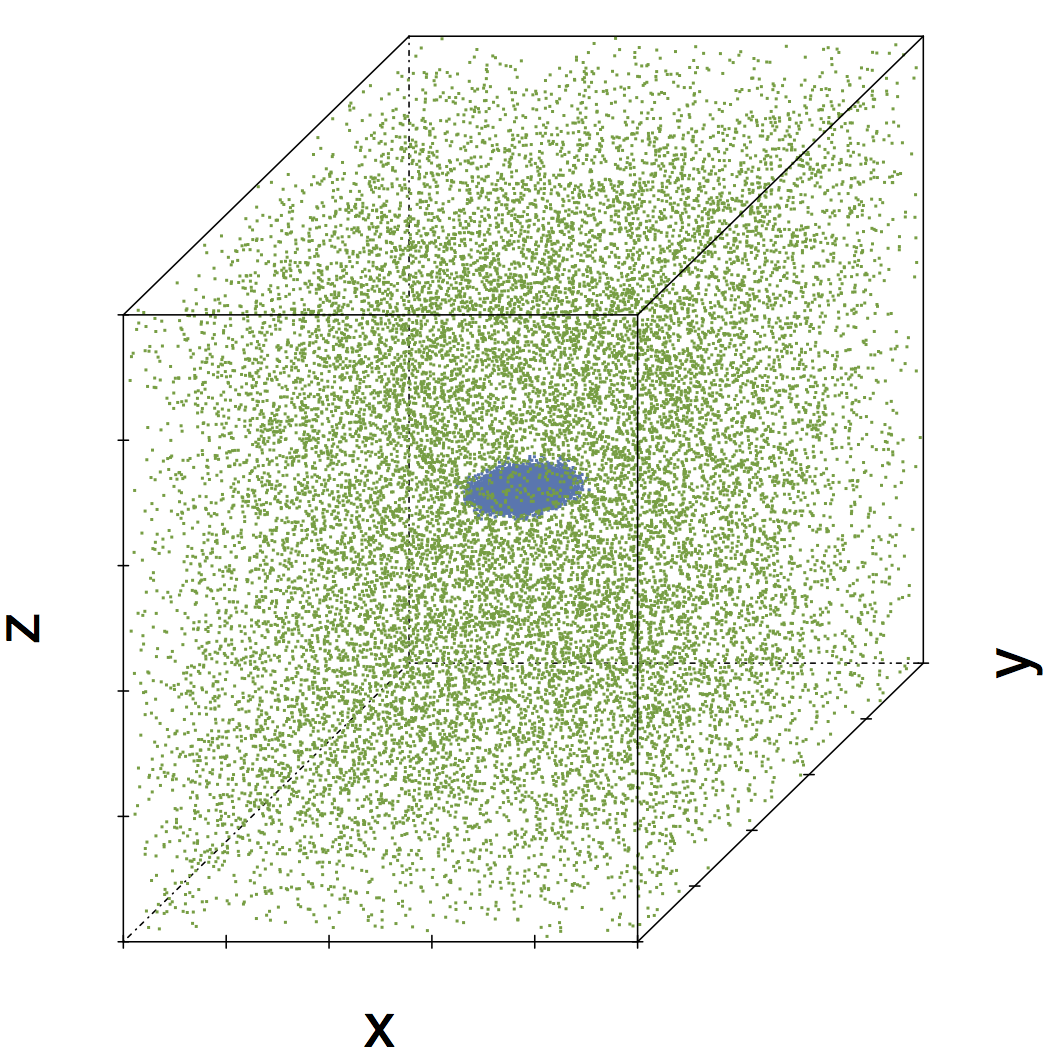
\includegraphics[width=\textwidth]{experiment/img/datasetplot_baakman_4_60000}
	\caption{Set \baakmanFour}
	\label{fig:3:simulated:datasets:baakman4}
\end{subfigure}	
% Baakman 5
\begin{subfigure}{0.23\textwidth}
	\centering
	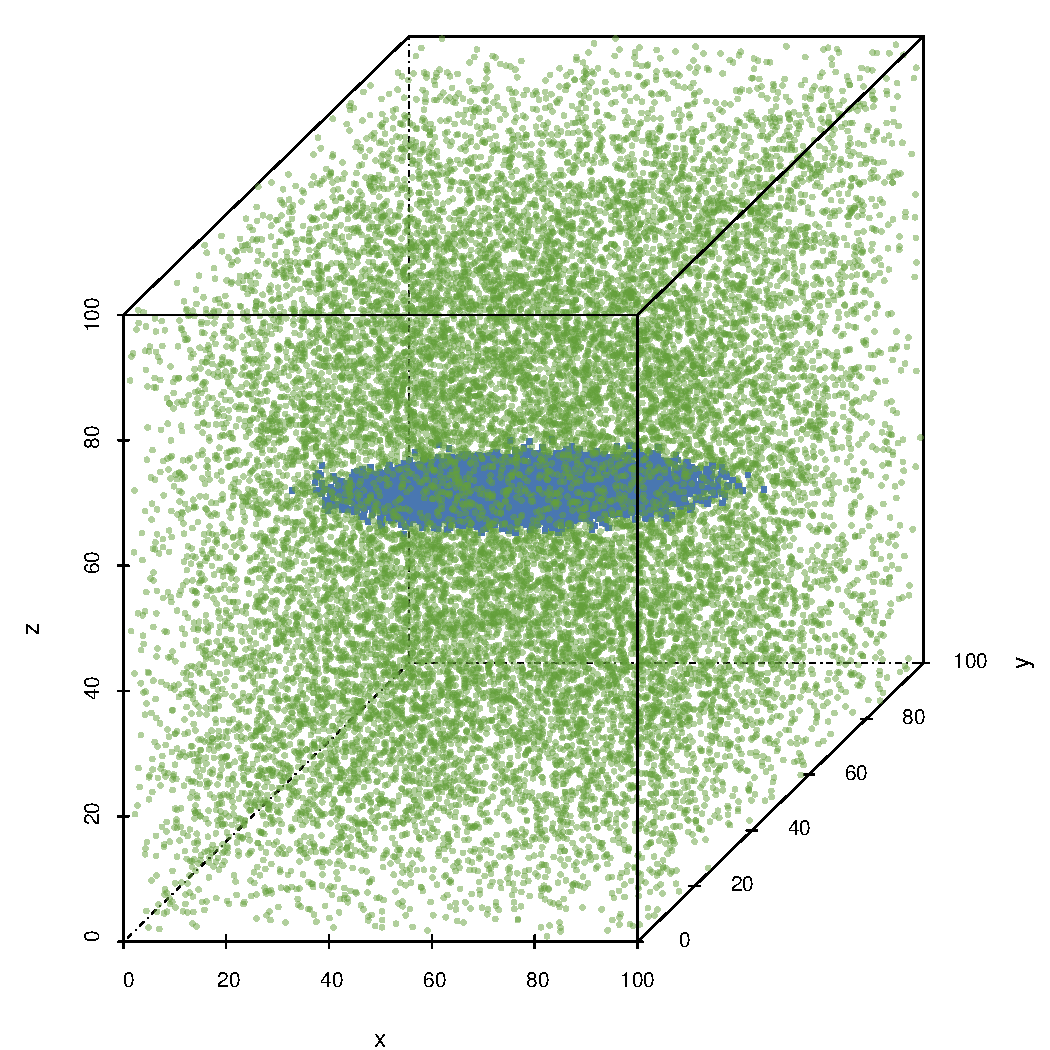
\includegraphics[width=\textwidth]{experiment/img/datasetplot_baakman_5_60000}
	\caption{Set \baakmanFive}
	\label{fig:3:simulated:datasets:baakman5}
\end{subfigure}	
	\caption{Scatter plot representation of the datasets defined in \cref{tab:experiment:singlesphere:sets}. The used colors correspond to those associated with the different components in \cref{tab:experiment:singlesphere:sets}.}
	\label{fig:experiment:singlesphere:sets}
\end{figure*}

\begin{table*}
	\centering
	%!TEX root = ../paper.tex

%!TEX root = ../paper.tex
\sisetup{
	table-format=5.0,
	scientific-notation=false,
	round-mode=places,
	round-precision=1,
	table-number-alignment=center
}
\begin{tabular}{@{}cclSl@{}}
\toprule
Set 			&~						& Component					& {Number} 	& Distribution\\
\midrule
% Ferdosi 1
\ferdosiOne 	&\legendComponentOne	& Trivariate Gaussian 		& 40000		& $\gaussDist{[50, 50, 50]}{\diag(11)}$\\
~ 				&\legendComponentNoise	& Uniform random background	& 20000		& $\uniformDist{[0, 0, 0]}{[100, 100, 100]}$\\
% Baakman 1
\hline
\baakmanOne		&\legendComponentOne	& Trivariate Gaussian 		& 40000		& $\gaussDist{[50, 50, 50]}{\diag([11, \sqrt{11}, \sqrt{11}])}$\\
~ 				&\legendComponentNoise	& Uniform random background	& 20000		& $\uniformDist{[0, 0, 0]}{[100, 100, 100]}$\\
% Baakman 4
\hline
\baakmanFour	&\legendComponentOne	& Trivariate Gaussian 		& 40000		& $\gaussDist{[50, 50, 50]}{\diag([11, 2 * \sqrt{11}, \rfrac{1}{2} \sqrt{11}])}$\\
~ 				&\legendComponentNoise	& Uniform random background	& 20000		& $\uniformDist{[0, 0, 0]}{[100, 100, 100]}$\\
% Baakman 5
\hline
\baakmanFive	&\legendComponentOne	& Trivariate Gaussian 		& 40000		& $\gaussDist{[50, 50, 50]}{\diag([11^2, 11, 1])}$\\
~ 				&\legendComponentNoise	& Uniform random background	& 20000		& $\uniformDist{[0, 0, 0]}{[100, 100, 100]}$\\
\bottomrule
\end{tabular}
	\caption{The datasets containing a single Gaussian distribution embedded in uniform noise. The column `Number' indicates for each component the number of patterns sampled from it. \gaussDist{\varMean}{\varCovarianceMatrix} denotes a Gaussian distribution with mean \varMean and covariance matrix \varCovarianceMatrix. A diagonal matrix with the values $x_1,\, \cdots,\, x_\varDim$ on the diagonal is represented as $\diag([x_1,\,\cdots,\,x_\varDim]])$, a scalar matrix with $x$ on the diagonal is shown as $\diag(x)$. \uniformDist{a}{b} denotes a uniform distribution with its minimum and maximum set to $a$ and $b$, respectively. The second column presents the symbol used to represent this component in plots throughout the paper.} 	
	\label{tab:experiment:singlesphere:sets}
\end{table*}

\Cref{fig:experiment:singlesphere:sets} shows a scatter plot representation of the datasets defined in \cref{tab:experiment:singlesphere:sets}. 

% General
The Gaussian components of these datasets progress from a sphere, \ie dataset \ferdosiOne, to an increasingly more elongated ellipsoid. This makes it possible to investigate the influence of how strongly elongated the distribution is, on the density estimate. 
	% Ferdosi One
	The first dataset is a simple spherical Gaussian distribution centered in a uniform random background. 
	% Baakman One
	The covariance matrix of the Gaussian component in \baakmanOne is created from \ferdosiOne by squaring one of the eigenvalues of the covariance matrix, and taking the square root of the other two eigenvalues, without changing the eigenvectors. The resulting covariance matrix defines an eigenellipse with the same volume as the one defined by \ferdosiOne.
	% Baakman Four
	The Gaussian component of dataset \baakmanFour changes the shape of the eigenellipse of the Gaussian component by lengthening one of the minor axes, and shortening the other.
	% Baakman Five
	In dataset \baakmanFive the Gaussian component is spread out more along the y-axis and less along the z-axis, than the Gaussian component in dataset \baakmanFour.

% Hypothesis
	% Ferdosi 1
	We expect the Modified Breiman Estimator and its shape-adaptive cousin to perform comparably on dataset \ferdosiOne, since due to the symmetric shape of the Gaussian distribution no advantage should be gained by using a shape-adaptive kernel. 
	% Baakman 1, 4, 5
	As the Gaussian distribution is more and more elongated, the advantages of using \sambe should become more pronounced. 